\documentclass{article}

% if you need to pass options to natbib, use, e.g.:
% \PassOptionsToPackage{numbers, compress}{natbib}
% before loading nips_2016
%
% to avoid loading the natbib package, add option nonatbib:
% \usepackage[nonatbib]{nips_2016}

\usepackage[final]{nips_2016}

\include{bibliography.bib}


% to compile a camera-ready version, add the [final] option, e.g.:
% \usepackage[final]{nips_2016}

\usepackage[utf8]{inputenc} % allow utf-8 input
\usepackage[T1]{fontenc}    % use 8-bit T1 fonts
\usepackage{hyperref}       % hyperlinks
\usepackage{url}            % simple URL typesetting
\usepackage{booktabs}       % professional-quality tables
\usepackage{amsfonts}       % blackboard math symbols
\usepackage{nicefrac}       % compact symbols for 1/2, etc.
\usepackage{microtype}      % microtypography
\usepackage{fontenc}
\usepackage[utf8]{inputenc}
\usepackage{mathtools}
\usepackage{float}

\title{Gaussian Processes and Portfolio Optimization}

\author{
  Nathaniel L. Diamant \\
  Department of Mathematics\\
  Harvey Mudd College\\
  \texttt{ndiamant@hmc.edu} \\
  \And Kyle Suver \\
  Department of Mathematics\\
  Harvey Mudd College\\
  \texttt{ksuver@hmc.edu} \\
}

\begin{document}

\maketitle

\begin{abstract}
  Portfolio optimization is a problem as old as the stock market. It has often been formulated as a Quadratic Program \cite{convex} that optimizes either for maximal returns or minimal portfolio variance with the other as a constraint. We reformulate the problem to simultaneously optimize variance and returns with a hyperparameter to control risk aversion. In order to predict returns and portfolio variance, we use Gaussian processes, which allow smooth data interpolation and regression with confidence bounds \cite{spectral}. Combining portfolio optimization and Gaussian Processes, we test on random stocks to demonstrate the viability of our algorithm.
\end{abstract}

\section{Introduction}
\label{intro}

The goal of this paper is to create an optimum short term stock portfolio.  Our approach is based on maximizing the Sharpe Ratio.  The Sharpe Ratio is defined as the expected return of a stock or portfolio divided by its standard deviation.  This has historically been considered as a measure of how ``good'' a stock is. We reformulate the portfolio optimization problem to maximize proxy measure for the Sharpe ratio.  We first attempted to compute the maximum of the log of the Sharpe Ratio, but as we will show, this created a non-convex optimization problem, which would be impractical for a short-term optimization problem.  

To fix this problem we will instead use a convex combination of the negative of the return value, and the positive of the variance value, and minimize this.  This means that we will be maximizing the return value and minimizing the variance of the stocks in our portfolio, trying different weights to balance returns and stability of the portfolio.

\subsection{Gaussian Processes (GPs)}

A Gaussian process is a collection of random variables, each of which has a joint Gaussian distribution.  Running the Gaussian process will generate a distribution over functions $f(x)$,
\begin{equation}
	f(x) \sim \mathcal{GP}(m(x), \kappa(x, x')
    \label{eqn:GP}
\end{equation}

where $x \in \mathcal{R}^P$ is an input variable, $m(x)$ is the mean function ($\mathbb{E}[f(x)]$) and $\kappa (\textbf{x}, \textbf{x}')$ is the covariance kernel.  

The kernel is a function which defines the distance between any two points in our data set. In our case we used the RBF kernel, also known as the Squared Exponential Kernel. It is the standard kernel people try because it yields smooth interpolation and easily interpretable variances. 

Any collection of Gaussian process functions has a joint Gaussian distribution, so from this method we can infer a posterior predictive distribution over Gaussian process functions, and analytically derive a marginal likelihood of the function values given the hyperparameters. \cite{spectral}


\subsection{Portfolio Optimization}

Modern portfolio theory defines a quadratic programming problem for optimizing a portfolio as
\begin{alignat*}{2}
    \text{minimize }   &   \textbf{w}^\top \mathbf{\Sigma} \textbf{w}\\
    \text{subject to } & \sum_i w_i E_i \geq R \\
    & \textbf{1}^\top \textbf{w} = 1 \\
    & \textbf{w} \underline{\succ} 0
\end{alignat*}
where $E_i$ are the expected values for our individual stocks, $\textbf{w}$ is the weights matrix, and $\mathbf{\Sigma}$ is the covariance matrix for our data. What this program is capturing is the idea that we want to minimize the correlations between the stocks we choose for our portfolio to make it diverse.  However we want to ensure that we are getting a positive return on our portfolio, so we add a constraint that the returns $\left(\sum_i w_i E_i \right)$ are at least some constant $R$.  

We decided to not use this same optimization problem, because it settles for having the expected returns simply be better than a constant, and we want to use the expected returns from our Gaussian process to give the best possible portfolio.  Because of this, we decided to change the optimization problem to a convex combination of the returns and variances, which captures the essence of the Sharpe ratio, but also allows a user to define whether they want their portfolio to focus more on diversity or expected returns.  


\section{Background}
\label{background}
The first step of our algorithm is to compute the average returns and covariances of our function using a Gaussian Process.  As stated in the introduction we used the RBF Kernel for our testing.  This kernel is defined as 
\begin{equation}
	\kappa (\textbf{x}, \textbf{x}') = \exp \left( - \frac{\|\textbf{x} - \textbf{x}' \|^2}{2\sigma^2} \right).
    \label{eqn:RBF}
\end{equation}
The results of using the RBF kernel on a stock can be seen in Figure~\ref{fig:GP}.

\begin{figure}[H]
  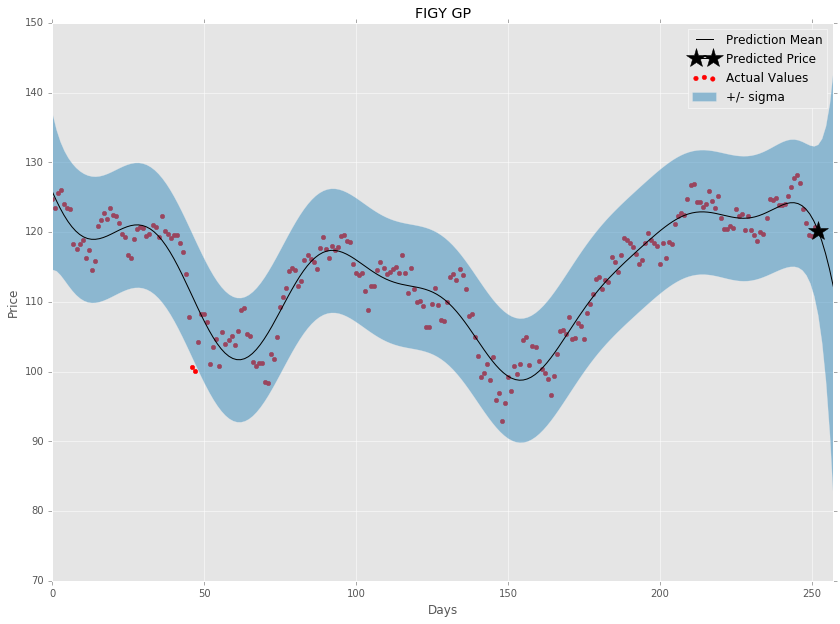
\includegraphics[scale=.5]{figy.png}
  \caption{A Gaussian process on FIGY with hyperparameters optimized by the GPy library.}
  \label{fig:GP}
\end{figure}

The next step is the portfolio optimization.  Part of our problem is reformulating this optimization problem is to reformulate the objective as to account for how high we want the returns.  Because we want our data to reflect the idea of the Sharpe Ratio, the best objective function we could use would be, using the same notation as above,
\begin{alignat*}{2}
    \text{minimize }   &   \textbf{E}^\top \textbf{w} (\textbf{w}^\top \mathbf{\Sigma} \textbf{w})^{-1}\\
    \text{subject to } 
    & \textbf{1}^\top \textbf{w} = 1 \\
    & \textbf{w} \underline{\succ} 0
\end{alignat*}
Because this captures the idea that our function is the Sharpe Ratio because we have the returns ($\textbf{E}^\top \textbf{w}$) times the inverse of the portfolio variance ($(\textbf{w}^\top \mathbf{\Sigma} \textbf{w})^{-1})$ which is like dividing them.  However this function is not feasible to use on a large data set because it is not convex.  Because of this we will redefine our optimization problem to be
\begin{equation}
\begin{array}{ll@{}ll}
\text{minimize}  & \displaystyle -\theta \textbf{E}^\top \textbf{w} + (1-\theta)\textbf{w}^\top \mathbf{\Sigma} \textbf{w} &\\
\text{subject to}& \displaystyle\textbf{1}^\top \textbf{w} = 1 \\
                 &  \textbf{w} \underline{\succ} 0                                     
\end{array}
\end{equation}
where $\theta$ is some constant where $0 \leq \theta \leq 1$. This objective fixes the issue of being non-convex by doing a convex combination of two things which we know to be convex.  While it doesn't give the exact measure of the Sharpe Ratio, it does take into account both the expected returns and variance.  We can then optimize the value of $\theta$ to ensure that we get the best possible return each time.  In addition, this gives the user control over how much they want their portfolio to be weighted by the returns or variance, so that a user could customize to an investment strategy based on preference for returns or stability.

\section{Experiments}
\label{exper}

We ran our formula against daily stock data that was scraped from Yahoo finance by an anonymous donor.  The data set had daily stock data starting in January 2000, for 7,420 different stocks.  In order to formulate tests for our data we needed to select samples of the stocks in our data set and run them with different $\theta$ values.  This allows us to find an optimal value for $\theta$. Which we could then use to test our data.  

In order to test our effectiveness on individual stocks, we cut the data into training and testing sets, then use the training data to predict the first data point in the testing set. We then compute the return we got with our prediction, add it to a list of returns, then repeat this by moving the point we just predicted into the training set and predicting the next point.  With the list of returns we get, we can multiply them all together to get the return over the time period we checked.

\subsection{100 day test}

\begin{figure}[H]
  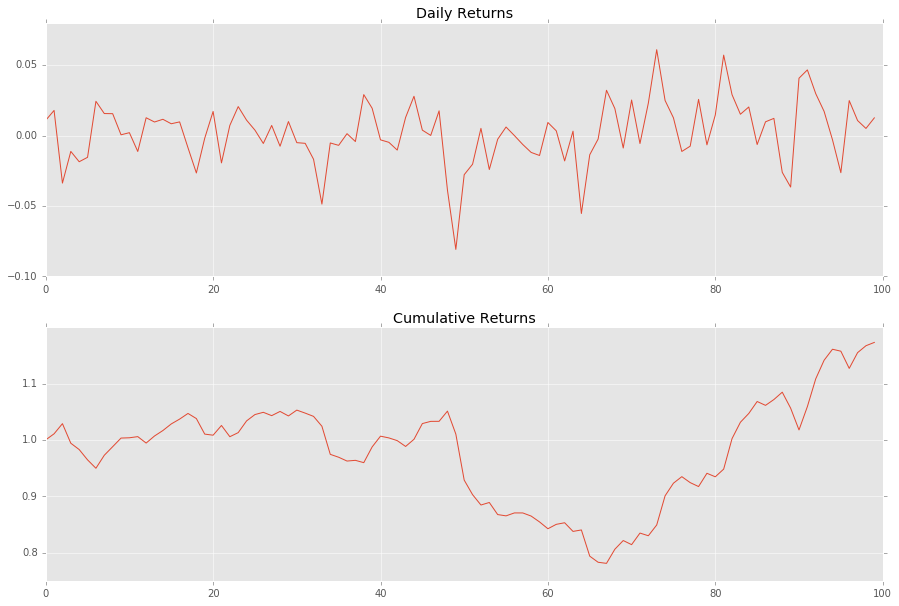
\includegraphics[scale=.5]{pointonereturns.png}
  \caption{A plot of the daily and cumulative returns of our algorithm when run on a random set of 100 stocks for 100 days.  The $\theta$ parameter was randomly chosen to be .1.}
  \label{fig:returns}
\end{figure}
In Figure~\ref{fig:returns}, we tested our data set over a 100 day period using 100 randomly selected stocks, simulating how our algorithm would perform in a real trading situation.  We selected the $\theta$ parameter to be .1 for the sake of testing, which means that the returns were weighted much less than the variances of the stocks.  This test resulted in an $18\%$ gain in our portfolio in 100 days, but the rise in price was not constant.  However if you look at the S\&P 500 for the period that we are predicting for (March to June 2016) the market does dip down at roughly the same point as our strategy, so it's not too surprising that we would lose money at this point. However, this is much more intense dip in price than the S\&P 500 took, but also a much bigger rise after the fact.

We believe that the reason our algorithm does poorly in a bear market because in this test, even if it believes it will take a loss, the algorithm still invests all of its money.

\subsection{Varying $\theta$}

We ran the algorithm on a single day with randomly selected stocks and then calculated the portfolio return and covariance with different values of $\theta$. We also include a dummy stock in the data that has zero variance and no returns to represent not investing the money. The results can be seen in Figure~\ref{fig:theta}

\begin{figure}
\begin{center}
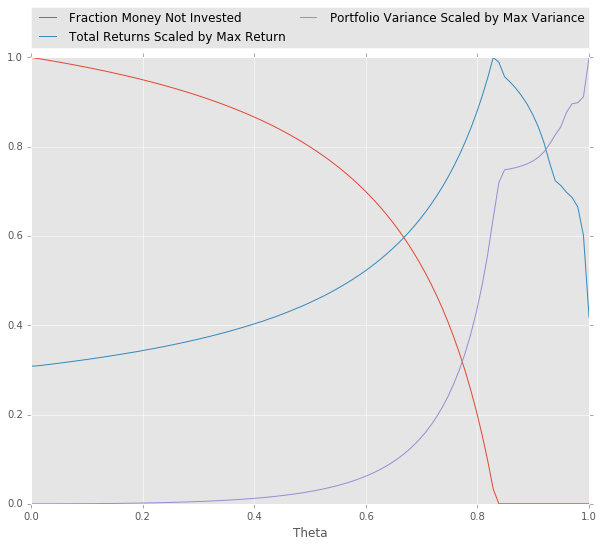
\includegraphics[width=.4\textwidth]{varytheta5.png}
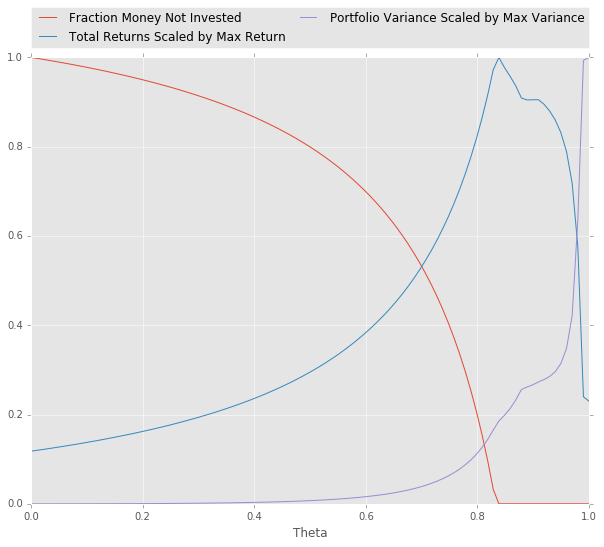
\includegraphics[width=.4\textwidth]{varytheta2.png}
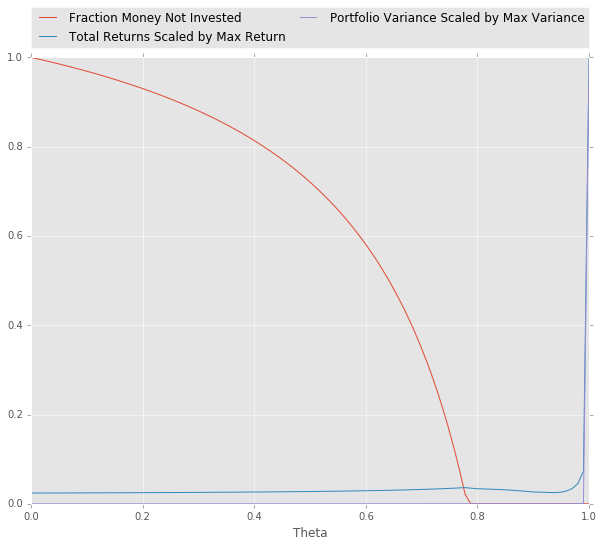
\includegraphics[width=.4\textwidth]{varytheta3.png}
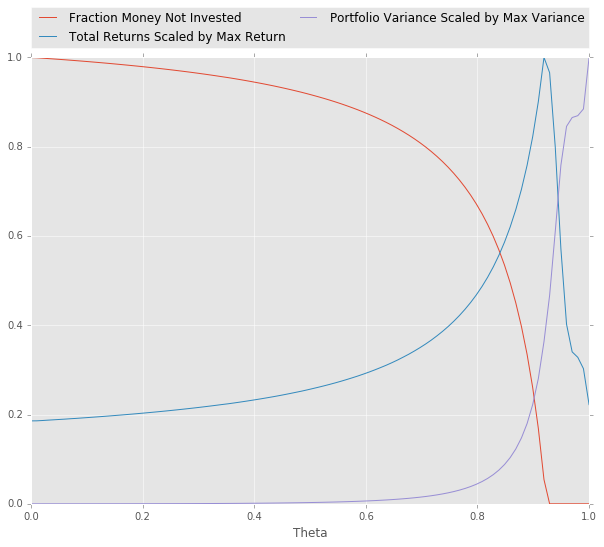
\includegraphics[width=.4\textwidth]{varytheta4.png}
\end{center}
\caption{How returns, non investment, and portfolio covariance vary with $\theta$}
\label{fig:theta}
\end{figure}

As expected, at $\theta = 0$, all of the money goes into the zero variance option of holding the money and when $\theta = 1$, all of the money goes into the stock with the highest predicted return, regardless of its variance. We notice some more interesting trends worth further investigation. It seems that when the money not invested hits zero, the returns are often maximized. We cannot explain this result, but could be a very valuable insight.

\subsection{Results}

The results that we got do end up having a surprising amount of sparsity.  On a small test we did of 48 stocks, we only had 12 stocks that we put more than $1\%$ of our investment into.  When we scale the number of stocks up to 1000, we get that only 2 stocks take up more than $1\%$ of our investment each and combined they make up more than $99\%$ of our investment. There are also only 16 stocks that take up more than $.1\%$ of our investment.  This is a useful result because it means we only have to invest our money into a few stocks each day, which will minimize the effect of market friction on our trading strategy.

While in some ways this is a positive result, it also might indicate an issue with how well the covariance optimization is working.  If we pick 2 stocks, even for a one day period, we most likely are not diversifying our portfolio as we would like.  However, our algorithm still is able to pick out stocks that are good enough that they can make up the majority of a portfolio and still be profitable, which is a good sign.

\subsection{Future Work}

There are several possible changes we could make to our algorithm to make it potentially more efficient.  

One of these would be to try using a Student-t Process instead of a Gaussian Process for prediction \cite{student-t}.  The benefit of this is that each data point would be represented as a Student-t distribution rather than a Gaussian distribution, and Stocks are generally considered to more closely follow the Student-t distribution.  It would also probably be worthwhile to attempt this problem with several other types of distributions, and see which one gives the best result.  

Another potential improvement would be to try out different Kernels instead of the RBF Kernel.  One that would be specifically good for this would be the Spectral Mixture Kernel. \cite{spectral} With this Kernel we would better capture the periodic and momentum behavior of the Stock market.

We also would like to find a better way to optimize our hyperparameter $\theta$.  Our current approach is to run it over multiple days with multiple stocks, and brute force search for the most successful thetas.  This is effective, but incredibly slow.  With this approach it is unreasonable to train $\theta$ for every stock that we have, over a reasonable number of days, which leads to a non-optimal value for $\theta$.  A simple solution would be to just run this on a bigger machine, because then we could calculate $\theta$ in more reasonable time. 

It would also be very important to find a better way to combine the covariance of the stock data and variance of the Gaussian Process.  Currently our approach is to create a weighted sum of covariance matrix and a diagonal matrix of the variances. However we chose a random weighting of the sums, because if we optimized the weightings, the run time would be made significantly slower. If we had a more powerful machine we could definitely optimize for this parameter and $\theta$, which would probably give a better result.

Finally, investigating why when the money invested in the dummy stock hits zero (Figure~\ref{fig:theta}), returns are maximized could be very interesting. Is there a deep mathematical explanation?

\newpage

\bibliographystyle{unsrt}
\bibliography{bibliography}

\end{document}
